\chapter{\;\;\;\;Program Verification}
\label{sec:program}

\section{Background}
\label{sec:program:background}

%% Since its origination in 1960s,
Hoare logic, since its origination in 1960s, has shown great success as a program verification technique and modularity is at the heart of it success.
In Hoare logic, for a given program $prog$, verifier tries to establish the following formula $\hoare{P}{prog}{Q}$.
This is called {\it Hoare triple} and means that if the $prog$ starts in a state satisfying the {\it precondition} $P$,
its returning state should satisfy the {\it postcondition} $Q$.
%% In other words, Hoare triple guarantees {\it partial correctness} which means that $Q$ holds {\it if} the program terminates (returns), but Hoare triple itself does not say anything about termination.
%% In other words, Hoare triple guarantees {\it partial correctness}; it does not say anything about termination.
Then, the following {\it sequence} (or sequential composition) rule holds.

\[
\infer
    {\hoare{P}{c_{0} ; c_{1}}{R}}
    {\deduce{\hoare{P}{c_{0}}{Q} \;\;\;\;\;\; \hoare{Q}{c_{1}}{R}}
      {\textsc{(Sequence)}}}
    %% {\deduce{\viewshift{Q'}{Q''}}
    %%   {\deduce{\viewshift{Q}{Q'}}
    %%     {\deduce{\textsc{(Trans)}\phantom{aa}}{\phantom{a}}}}}
\]

\noindent The rule says that two Hoare triples can be composed as long as the former's postcondition coincides with the latter's precondition. Thanks to this sequence rule, the verifier can modularly verify each instruction of the program and then compose them to establish whole program correctness.



%%% plcc 120p
%%% VC 40p
%% \todo{앞의 sequence rule하고 연결이 안됨. 연결하는 내용 추가 (기본적으로 sequence rule하고 똑같은거다)}
Modern higher-order variants of Hoare logic\cite{VST,appel:plcc} supports another useful modular reasoning principle, which is written below (simplified for presentation purpose).%, but justifying it accompanies much complexity and it only works for partial correctness.
%% The rule (simplified for presentation purpose) is as follows.
\[
\infer
    %% {\hoare{P_{f}}{f}{Q_{f}} \;\;\;\;\;\;\; \hoare{P_{g}}{g}{Q_{g}}}
    %% {\infer
    %%   {\hoare{P_{g}}{g}{Q_{g}}}
    %%   {\hoare{P_{f}}{f}{Q_{f}}}
    %%   \;\;\;\;\;\;
    %%  \infer
    %%   {\hoare{P_{f}}{f}{Q_{f}}}
    %%   {\hoare{P_{g}}{g}{Q_{g}}}}
    {\deduce{\hoare{P_{g}}{\code{g}}{Q_{g}}}{\hoare{P_{f}}{\code{f}}{Q_{f}}}}
    {\deduce{\hoare{P_{f}}{\code{call} \; \code{f}}{Q_{f}} \implies \hoare{P_{g}}{\code{g}}{Q_{g}}}
            {\deduce{\hoare{P_{g}}{\code{call} \; \code{g}}{Q_{g}} \implies \hoare{P_{f}}{\code{f}}{Q_{f}}}
                    {\textsc{(Call)}}}
    }
    %% {\deduce{(\hoare{P_{f}}{f}{Q_{f}} \land \hoare{P_{g}}{g}{Q_{g}}) \implies \hoare{P_{g}}{g}{Q_{g}}}
    %%         {(\hoare{P_{f}}{f}{Q_{f}} \land \hoare{P_{g}}{g}{Q_{g}}) \implies \hoare{P_{f}}{f}{Q_{f}}}
    %% }
\]

\noindent When verifying two mutually recursive functions \code{f} and \code{g}, this reasoning principle allows one to verify \code{f} assuming the specification of \code{g} and vice versa.
Then, together with the sequence rule, one can pass by $\code{call} \; \code{f}$ (and $\code{call} \; \code{g}$, respectively) instead of going through its body.
The principle is seemingly unsound because it is a circular reasoning, but %(with a little fix)
it is indeed sound. %%because we are proving only the partial correctness.
In order to justify the principle, a technique called {\it step-index} is employed.
With this, it is sufficient to verify that \code{f}'s specification holds until $k+1$ steps assuming the specification of \code{g} holds until $k$ steps and vice versa.
Then, by using induction on the step-index $k$, one can show that $f$ and $g$'s specifications hold for any finite number of steps, which is sufficient because Hoare triple requires only the {\it partial correctness}.
%% \footnote{Actually, the principle is unsound for total correctness. For an instance, given $\code{f} \defeq \code{g()}$ and $\code{g} \defeq \code{f()}$, one would be able to prove \hoare{True}{\code{f}}{r . r = 42} and \hoare{True}{\code{g}}{r . r = 42}.
%%   These triples mean \code{f} and \code{g} terminates with return value $42$, and these are wrong. }
Partial correctness means that it does not say anything about termination; recall that Hoare triple requires the postcondition to hold {\it if} it happens to terminate.
%% Recall that Hoare triple requires the postcondition to hold {\it if} it happens to terminate; in other words, Hoare triple does not say anything about termination itself so are called partial correctness.
%% Partial correctness means that Hoare triple guarantees postcondition {\it if} it happens to terminate and does not say anything about termination itself.

\section{Problems}
\label{sec:program:problem}

However, those modern variants of Hoare logic also have few drawbacks.
First, the step-index complicates the underlying model, which makes soundness result (or even the meaning of a Hoare triple) esoteric.
Second, it supports only partial correctness (\ie cannot prove termination).
In fact, if we change the meaning of Hoare triple to guarantee {\it total correctness} (\ie both the postcondition and termination), the call rule becomes unsound.
\footnote{Here is a simple counter example: $\code{f} := \code{call} \; \code{f}$. Here, one can prove arbitrary pre/postcondition on $\code{f}$ by using the call rule, which in turn implies that $\code{f}$ terminates. This is contradiction.}
%% \footnote{\cite{jung:irisjfp} \todo{Iris jfp 도 full functional, contextual refinement 지원한다고 써놓기는 했는데 이게 total weakestpre라서 invariant 못쓸거임}}
Therefore, to prove total correctness, one needs to employ a separate tool.
%% \footnote{There are also some variants of Hoare logic which proves total correctness, but it is too stringent to be realistic. Consider the verification of library code where clients are unknown.
%% Using total Hoare logic here will rule out potential non-terminating clients (e.g., web server).}
Third, its adequacy results hold only when the whole program is verified with the same Hoare logic.
This is restrictive because we often want to verify each module with different tools (such as model checker).
Finally, it cannot verify a program that communicates with the outside world. Think of a simple REPL, a web server, or an operating system; it is even unclear how to write a Hoare triple for such a program.
%% Moreover, consider verification of a web server or an operating system; it is not realistic to enforce clients or user-level applications to be formally verified with the same Hoare logic.
%% \even{step-index complicates underlying model, spec is very hard to understand, etc...}
%% Third, \todo{gradual abstraction} ...

\section{TODO}
\label{sec:program:solution}

\section{Future Works}
\label{sec:program:future}
%% automation 이야기... layered approach

\section{Related Works}
\label{sec:program:related}

\todo{TODO}

\myparagraph{\certikos}

\myparagraph{Armada}

\myparagraph{Establishing Refinement with Hoare Logic}

\myparagraph{Transfinite Step Indexing}

\myparagraph{Other Variants of Hoare Logic}
Nikhil swamy



%% Since its origination in 1960s,
Hoare logic, since its origination in 1960s, has shown great success as a program verification technique and modularity is at the heart of it success.
In Hoare logic, for a given program $prog$, verifier tries to establish the following formula $\hoare{P}{prog}{Q}$.
This is called {\it Hoare triple} and means that if the $prog$ starts in a state satisfying the {\it precondition} $P$,
its returning state should satisfy the {\it postcondition} $Q$.
%% In other words, Hoare triple guarantees {\it partial correctness} which means that $Q$ holds {\it if} the program terminates (returns), but Hoare triple itself does not say anything about termination.
%% In other words, Hoare triple guarantees {\it partial correctness}; it does not say anything about termination.
Then, the following {\it sequence} (or sequential composition) rule holds.

\[
\infer
    {\hoare{P}{c_{0} ; c_{1}}{R}}
    {\deduce{\hoare{P}{c_{0}}{Q} \;\;\;\;\;\; \hoare{Q}{c_{1}}{R}}
      {\textsc{(Sequence)}}}
    %% {\deduce{\viewshift{Q'}{Q''}}
    %%   {\deduce{\viewshift{Q}{Q'}}
    %%     {\deduce{\textsc{(Trans)}\phantom{aa}}{\phantom{a}}}}}
\]

\noindent The rule says that two Hoare triples can be composed as long as the former's postcondition coincides with the latter's precondition. Thanks to this sequence rule, the verifier can modularly verify each instruction of the program and then compose them to establish whole program correctness.



%%% plcc 120p
%%% VC 40p
\todo{앞의 sequence rule하고 연결이 안됨. 연결하는 내용 추가 (기본적으로 sequence rule하고 똑같은거다)}
Modern higher-order variants of Hoare logic\cite{VST,appel:plcc} supports another useful modular reasoning principle, which is written below (simplified for presentation purpose).%, but justifying it accompanies much complexity and it only works for partial correctness.
%% The rule (simplified for presentation purpose) is as follows.
\[
\infer
    %% {\hoare{P_{f}}{f}{Q_{f}} \;\;\;\;\;\;\; \hoare{P_{g}}{g}{Q_{g}}}
    %% {\infer
    %%   {\hoare{P_{g}}{g}{Q_{g}}}
    %%   {\hoare{P_{f}}{f}{Q_{f}}}
    %%   \;\;\;\;\;\;
    %%  \infer
    %%   {\hoare{P_{f}}{f}{Q_{f}}}
    %%   {\hoare{P_{g}}{g}{Q_{g}}}}
    {\deduce{\hoare{P_{g}}{\code{g}}{Q_{g}}}{\hoare{P_{f}}{\code{f}}{Q_{f}}}}
    {\deduce{\hoare{P_{f}}{\code{f}}{Q_{f}} \implies \hoare{P_{g}}{\code{g}}{Q_{g}}}
            {\hoare{P_{g}}{\code{g}}{Q_{g}} \implies \hoare{P_{f}}{\code{f}}{Q_{f}}}
    }
    %% {\deduce{(\hoare{P_{f}}{f}{Q_{f}} \land \hoare{P_{g}}{g}{Q_{g}}) \implies \hoare{P_{g}}{g}{Q_{g}}}
    %%         {(\hoare{P_{f}}{f}{Q_{f}} \land \hoare{P_{g}}{g}{Q_{g}}) \implies \hoare{P_{f}}{f}{Q_{f}}}
    %% }
\]

\noindent When verifying two mutually recursive functions \code{f} and \code{g}, this reasoning principle allows one to verify \code{f} assuming the specification of \code{g} and vice versa.
The principle is seemingly unsound because it is a circular reasoning, but (with a little fix%% \todo{is this fix essential?}
) it is indeed sound. %%because we are proving only the partial correctness.
In order to justify the principle, a technique called {\it step-index} is employed.
With this, it is sufficient to verify that \code{f}'s specification holds until $k+1$ steps assuming the specification of \code{g} holds until $k$ steps and vice versa.
Then, by using induction on the step-index $k$, one can show that $f$ and $g$'s specifications hold for any finite number of steps, which is sufficient because Hoare triple requires only the {\it partial correctness}.
\footnote{Actually, the principle is unsound for total correctness. For an instance, given $\code{f} \defeq \code{g()}$ and $\code{g} \defeq \code{f()}$, one would be able to prove \hoare{True}{\code{f}}{r . r = 42} and \hoare{True}{\code{g}}{r . r = 42}.
  These triples mean \code{f} and \code{g} terminates with return value $42$, and these are wrong. }
Partial correctness means that Hoare triple guarantees postcondition {\it if} it happens to terminate and does not say anything about termination itself.




However, Hoare logic also has few drawbacks.
First, step-index complicates the underlying model, and this in turn makes soundness result (or even the meaning of a Hoare triple) esoteric.
Second, it has poor support for termination proof.
Most variants of Hoare logic proves only the partial correctness.
%% \footnote{\cite{jung:irisjfp} \todo{Iris jfp 도 full functional, contextual refinement 지원한다고 써놓기는 했는데 이게 total weakestpre라서 invariant 못쓸거임}}
Thus, for proving {\it total correctness}, which guarantees both the postcondition and termination, one usually proves termination separately using another tool.
\footnote{There are also some variants of Hoare logic which proves total correctness, but it is too stringent to be realistic. Consider the verification of library code where clients are unknown.
Using total Hoare logic here will rule out potential non-terminating clients (e.g., web server).}
Third, its adequacy results holds only when the whole program is verified with the same Hoare logic. This is restrictive because we often want to verify each module with different tools (such as model checker).
Moreover, consider verification of an web server or an operating system; it is not realistic to enforce clients or user-level applications to be formally verified with the same Hoare logic.
%% \todo{step-index complicates underlying model, spec is very hard to understand, etc...}
%% Third, \todo{gradual abstraction} ...








Our approach supports modular reasoning principle in the presence of mutual recursion, but does not suffer from aforementioned drawbacks.
%% Now, we will explain what our approach is
First, we write a specification as a {\it module}, not in C but in abstract mathematical state transition system. %%simpler, abstract
For an instance, if we have a C module computing Fibonacci number employing dynamic programming technique, its specification module directly returns $\mathrm{Fib}(\code{n})$ for an argument \code{n} where $\mathrm{Fib}$ is a Gallina function.
Then, each implementation module (written in C or assembly) is verified against its specification module using open simulations, thus implying RUSC relation.
The challenge here is: How to utilize the specifications of other modules even though what we are proving is RUSC, which quantifies over an arbitrary context?
Our key idea is that, instead of directly assuming the specifications of other modules, we carefully write each specification module to give an illusion as if we are assuming specifications of other modules.
Specifically, in $f_{spec}$, it calls $g$ and then check if $g$ returns the expected value. If so, it will proceed, but if not, it will trigger UB.
As a result, when verifying $f_{spec} \rusc_\rels f_{impl}$ one needs to proceed the simulation proof only when $g$ behaves as expected, because otherwise the proof is trivial.
Finally, after each module's verification is over, we can {\it merge} these modules to form $fg_{spec}$ and remove the potential source of UB.

%% 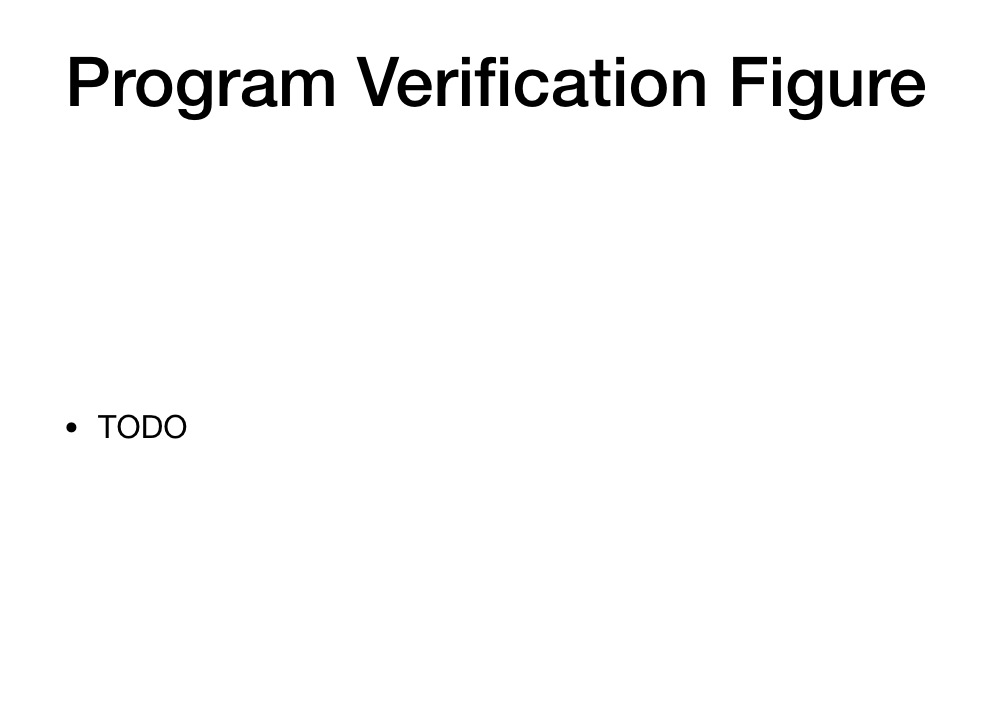
\includegraphics[width=0.6\linewidth]{fig-program-verif.png}

\noindent Now we explain why our approach does not suffer from the drawbacks.
First and foremost, by passively modeling the expected behavior of other modules with UB, we don't have any circularity in our reasoning. Therefore, we don't need step-index and can use RUSC framework without any problem.
Second, we trivially support total correctness because the notion of behavior is termination-sensitive.
Third, we don't impose any restrictions on the client module because RUSC quantifies over an arbitrary context.


















\todo{revise}
In \Cref{sec:overview-verification} we presented how to achieve compositional compiler correctness
%% ---namely adequacy, horizontal compositionality, and vertical compositionality---
in our framework.  In this section we present what our framework additionally offers about compiler and
program verification: verifying more advanced compiler optimizations with module-local
invariants (\Cref{sec:overview-modulelocal:compiler}) and verifying program modules against their
mathematical specification modules (\Cref{sec:overview-modulelocal:program} and \Cref{sec:overview-modulelocal:utod}).
\revision{To the best of our knowledge, our framework is the
first, in the context of \cc{}, that is capable of verifying
the \emph{mutually recursive} example presented in \Cref{sec:overview-modulelocal:program}.}



\subsection{Verification against Specification Modules}
\label{sec:overview-modulelocal:program}

\begin{figure}[t]
\makebox[\linewidth]{\makebox[1.1\linewidth]{
\begin{minipage}{1.1\linewidth}
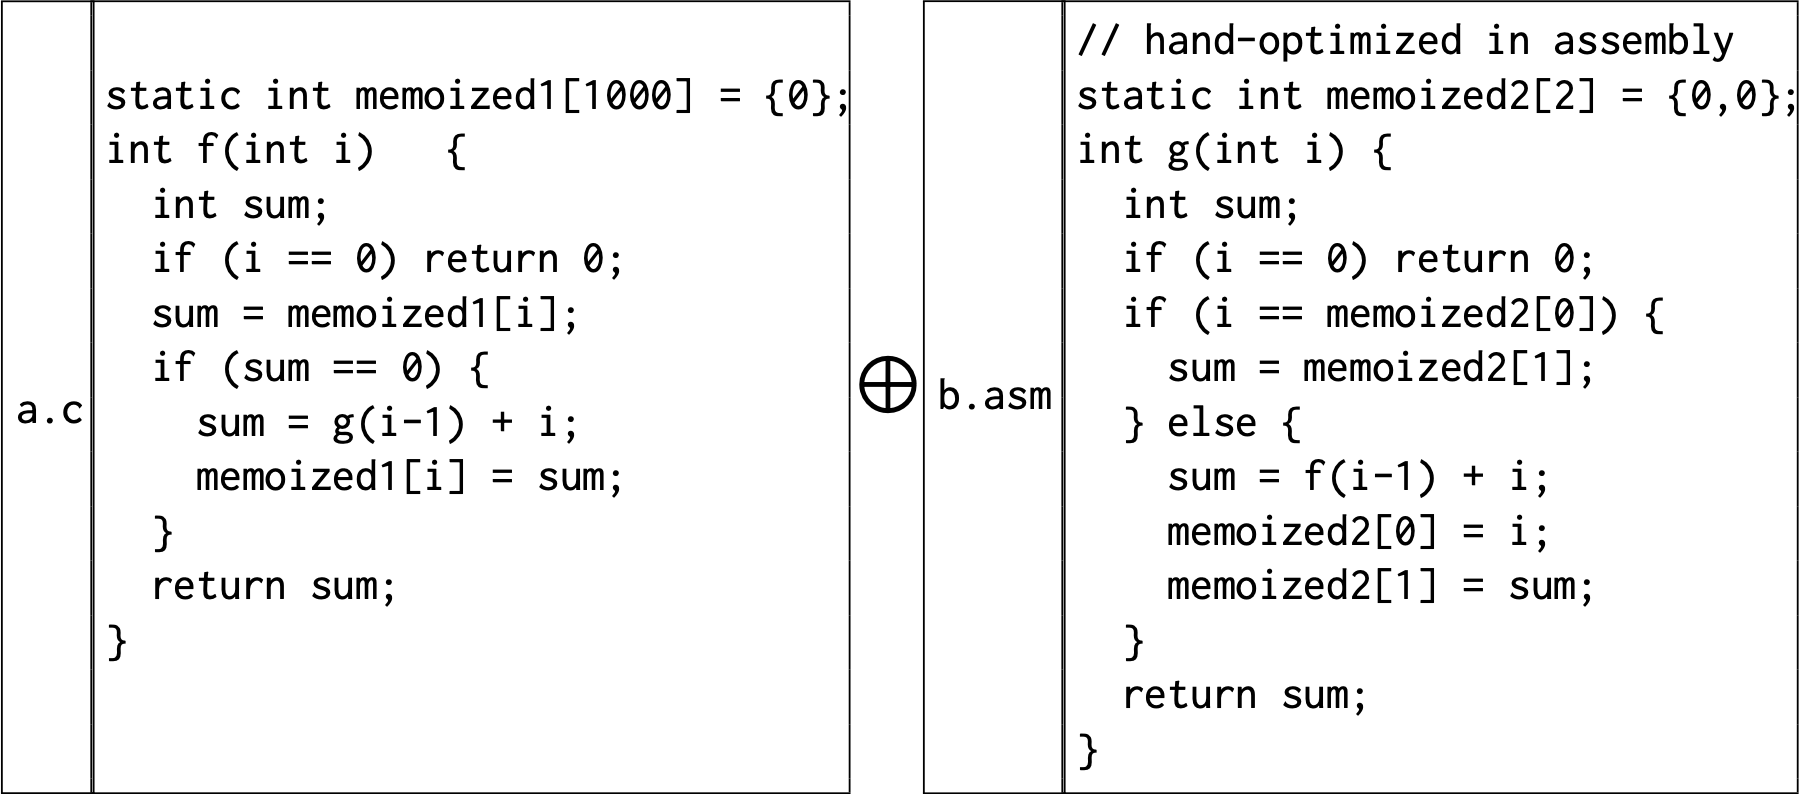
\includegraphics[width=1\linewidth]{images/mutsum1.png}
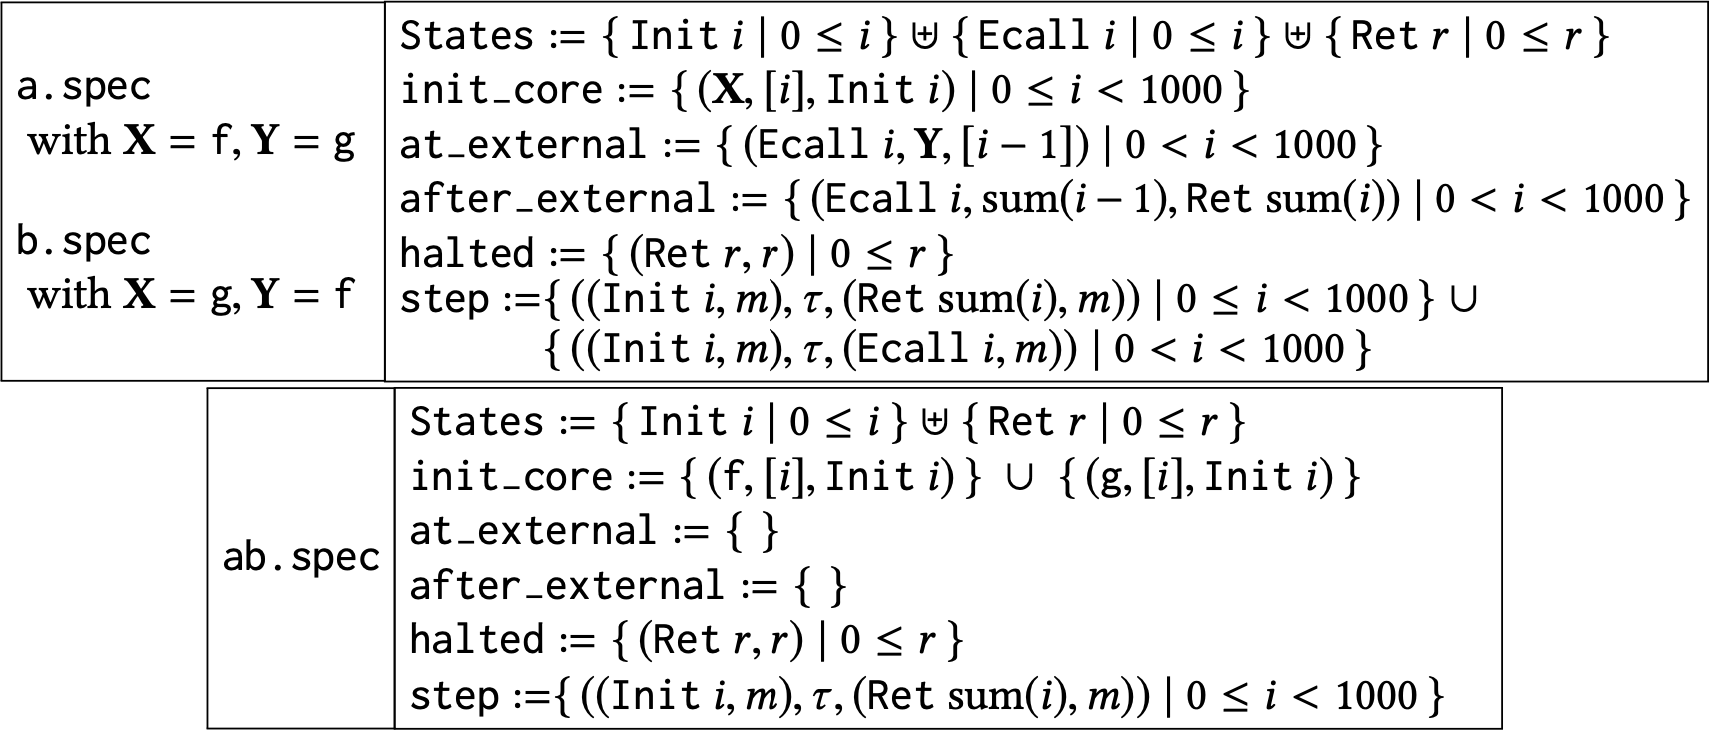
\includegraphics[width=1\linewidth]{images/mutsum2.png}
\end{minipage}
}}
\end{figure}

%% \begin{figure}[t]
%% \fbox{\begin{minipage}{1.15pc}\mbox{}\\[27.25mm]$\texttt{a.c}$\\[23.35mm]\mbox{}\end{minipage}}
%% \hspace*{-1.9mm}
%% \begin{minipage}{0.423\textwidth}
%% \begin{Verbatim}[frame=single]

%% static int memoized1[1000] = {0};
%% int f(int i)   {
%%   int sum;
%%   if (i == 0) return 0;
%%   sum = memoized1[i];
%%   if (sum == 0) {
%%     sum = g(i-1) + i;
%%     memoized1[i] = sum;
%%   }
%%   return sum;  
%% }


%% \end{Verbatim}
%% \end{minipage}
%% \hspace*{-2.0mm}
%% $\mbox{}~\mathlarger{\mathlarger{\mathlarger{\mathlarger{\mathlarger{\llink}}}}}~\mbox{}$
%% \hspace*{-2.2mm}
%% \fbox{\begin{minipage}{2.05pc}\mbox{}\\[26.21mm]$\texttt{b.asm}$\\[24.41mm]\mbox{}\end{minipage}}
%% \hspace*{-1.9mm}
%% \begin{minipage}{0.41\textwidth}
%% \begin{Verbatim}[frame=single]
%% // hand-optimized in assembly
%% static int memoized2[2] = {0,0};
%% int g(int i) {
%%   int sum;
%%   if (i == 0) return 0;
%%   if (i == memoized2[0]) {
%%     sum = memoized2[1];
%%   } else {
%%     sum = f(i-1) + i;
%%     memoized2[0] = i;
%%     memoized2[1] = sum;
%%   }
%%   return sum;
%% }
%% \end{Verbatim}
%% \end{minipage}
%% \\
%% \mbox{\fbox{\begin{minipage}{6.5pc}\mbox{}\\[2.13mm]$\texttt{a.spec}$ \\$\text{   with} ~ \textbf{X} = \texttt{f}, \textbf{Y} = \texttt{g}$\\[3.5mm]
%%       $\texttt{b.spec}$\\ $\text{   with} ~ \textbf{X} = \texttt{g}, \textbf{Y} = \texttt{f}$\\[0.33mm]\mbox{}\end{minipage}}
%% \hspace*{-1.9mm}
%% \fbox{\begin{minipage}{0.72\textwidth}
%%     $
%%   \texttt{States} := \setof{ \texttt{Init}\ i \ | \ 0 \leq i } \uplus \setof{ \texttt{Ecall} \ i\  |\  0 \leq i } \uplus \setof{ \texttt{Ret}\  r\  | \ 0 \leq r } \\
%%   \texttt{init\_core} := \setof{ (\textbf{X}, [i], \texttt{Init}\  i) \ |\  0 \leq i < 1000 } \\
%%   \texttt{at\_external} := \setof{ (\texttt{Ecall} \ i, \textbf{Y}, [i-1])\  |\  0 < i < 1000 } \\
%%   \texttt{after\_external} := \setof{ (\texttt{Ecall} \ i, \textrm{sum}(i-1), \texttt{Ret} \ \textrm{sum}(i))\  |\  0 < i < 1000 } \\
%%   \texttt{halted} := \setof{ (\texttt{Ret}\  r, r) \ |\  0 \leq r } \\
%%   \begin{aligned}
%%     \texttt{step} :=& \setof{ ((\texttt{Init} \ i, m), \tau, (\texttt{Ret}\  \textrm{sum}(i), m))\  |\  0 \leq i < 1000 } \ \cup \\[-1.5mm]
%%     &\setof{ ((\texttt{Init} \ i, m), \tau, (\texttt{Ecall}\  i, m))\  |\  0 < i < 1000 }\\[-1mm]
%%   \end{aligned}
%%   $
%% \end{minipage}}}
%% \\
%% \mbox{\fbox{\begin{minipage}{2.9pc}\mbox{}\\[8.73mm]$\texttt{ab.spec}$\\[6.93mm]\mbox{}\end{minipage}}
%% \hspace*{-1.9mm}
%% \fbox{\begin{minipage}{0.60\textwidth}
%%     $
%%   \texttt{States} := \setof{ \texttt{Init}\ i \ | \ 0 \leq i } \uplus \setof{ \texttt{Ret}\  r\  | \ 0 \leq r } \\
%%   \texttt{init\_core} := \setof{ (\texttt{f}, [i], \texttt{Init}\  i) } \ \cup \  \setof{ (\texttt{g}, [i], \texttt{Init}\  i) } \\
%%   \texttt{at\_external} := \setof{ } \\
%%   \texttt{after\_external} := \setof{ } \\
%%   \texttt{halted} := \setof{ (\texttt{Ret}\  r, r) \ |\  0 \leq r } \\
%%   \begin{aligned}
%%     \texttt{step} :=& \setof{ ((\texttt{Init} \ i, m), \tau, (\texttt{Ret}\  \textrm{sum}(i), m))\  |\  0 \leq i < 1000 }\\[-1mm]
%%   \end{aligned}
%%   $
%% \end{minipage}}}
%% \caption{The \code{mutual-sum} example}
%% \label{fig:modulelocal}
%% \end{figure}


\Cref{fig:modulelocal} shows a C module, \texttt{a.c}; a handwritten
assembly module, \texttt{b.asm} (presented in C syntax for
readability); their open specification modules, \texttt{a.spec} and
\texttt{b.spec}; and the combined closed specification module
\texttt{ab.spec}.  Both functions \texttt{f} in \texttt{a.c} and
\texttt{g} in \texttt{b.asm} mutually recursively compute the
summation from $0$ up to the given argument integer $i$ (denoted
$\mathrm{sum}(i)$), performing different memoization optimizations.
The function \code{f} memoizes the result of \code{f(i)} in the static
variable \code{memoized1[i]}, which is initialized with zero
representing invalid value.  The function call \code{f(i)} first reads
the memoized value, and returns it if it is valid; otherwise, it
calculates, memoizes, and returns \code{g(i-1)}, expected to be
$\mathrm{sum}(\code{i}-1)$, plus \code{i}.  On the other hand, the
function \code{g} memoizes only the result of the latest call
\code{g(i)} with the index \code{i}, where \code{memoized2[0]} =
\code{i} and \code{memoized2[1]} = \code{g(i)}.  The code of \texttt{g}
is self-explanatory under the assumption that the call \code{f(i-1)}
returns $\mathrm{sum}(\code{i}-1)$.

%% we have $\code{g(memoized[0])} = \code{memoized[1]}$.
%% The function \code{g(i)} is the same with
%% \code{f(i)}, except for memoization scheme, the callee of recursion,
%% and the language.

%% Our framework is flexible on the choice of languages to the degree that a module's (open)
%% specification can be represented as another module written in Coq's Gallina language.  Such
%% specification module facilitates modular verification of multi-language programs, as illustrated in
%% the example presented in \Cref{fig:modulelocal}.

%% Both of the function \code{f(i)} in the module \code{a.c} and \code{g(i)} in \code{b.asm} compute
%% $\textrm{sum}(\code{i})$, which is the summation from 1 to \code{i}, but with memoization and mutual
%% recursion on each other.\footnote{The module \code{b.asm} is written in hand-optimized assembly, but
%%   for presentational purposes we present it in C syntax.}  The module \code{a.c} memoizes the result
%% of \code{f(i)} in \code{memoized[i]}, which is initialized with zero representing invalid value.
%% The function \code{f(i)} first reads the memoized value, and returns it if valid; otherwise, it
%% calculates, memoizes, and then returns the summation of \code{g(i-1)}---which is expected to be
%% $sum(\code{i-1})$---and \code{i}.  On the other hand, \code{b.asm} memoizes only one result of
%% \code{g()}: we have $\code{g(memoized[0])} = \code{memoized[1]}$.  The function \code{g(i)} is the
%% same with \code{f(i)}, except for memoization scheme, the callee of recursion, and the language.


The open specification modules \texttt{a.spec} and \texttt{b.spec} are
the same except that the names of the internal and external functions
are swapped. This is natural because the two functions \code{f} and
\code{g} compute the same summation. The open specification
\texttt{a.spec} is an abstract, nondeterministic, version of the
function \texttt{f} in \texttt{a.c} including all the observable
behaviors of \texttt{f}.  It has three kinds of states,
$\code{Init}~i$, $\code{Ecall}~i$ and $\code{Ret}~r$, representing the
initial state with argument $i$, the call state executing
$\code{g}(i-1)$, and the halt state returning $r$, respectively. Then
\code{init\_core} starts with $\code{Init}~i$ when \texttt{f} is
invoked with argument $i$ if $0 \le i < 1000$, otherwise UB;
\code{at\_external} recognizes $\code{Ecall}~i$ as the state invoking
\texttt{g} with $i-1$; \code{after\_external} transitions
from $\code{Ecall}~i$ to $\code{Ret}~\mathrm{sum}(i)$ only
when the return value from the external call $\texttt{g}(i-1)$
is $\mathrm{sum}(i-1)$, otherwise UB, which
means that this module gives a conditional specification under the
assumption that $\texttt{g}(i)$ returns $\mathrm{sum}(i)$;
\code{halted} recognizes $\code{Ret}~r$ as the halted state returning
$r$; and finally $\code{step}$ transitions from $\code{Init}~i$ to
either $\code{Ret}~\mathrm{sum}(i)$ or $\code{Ecall}~i$
nondeterministically (without updating the memory), where the former
abstracts reading from memoization and the latter recursively
computing the sum. The same applies to \texttt{b.spec}.
Finally, the combined specification \code{ab.spec} does not make any
external function call and simply returns the summation.

Then, we perform our verification as follows.
First, we prove $\texttt{a.spec} \rusc_\rels \texttt{a.c}$
using memory injections with the following invariant:\\
%% \[
\mbox{}\hfill$\forall 0 \le i < 1000,~
\code{memoized1}[i] = 0 \lor \code{memoized1}[i] = \mathrm{sum}(i)~.$\hfill\mbox{}
%% \]
\\
Second, we prove $\texttt{b.spec} \rusc_\rels \texttt{b.asm}$
using memory injections with the following invariant:\\
%% \[
\mbox{}\hfill$
\exists 0 \le i < 1000,~
\code{memoized2}[0] = i \land \code{memoized2}[1] = \mathrm{sum}(i)~.
$\hfill\mbox{}
%% \]
\\
Finally, we prove $\texttt{ab.spec} \rusc_\rels \texttt{a.spec} \llink
\texttt{b.spec}$ using the memory identity.
\revision{Note that $\rels$ is the set containing open simulations with the three memory relations
  used in the above verification
  (\ie memory injections with the two invariants above and the memory identity).}

%% The module \code{ab.spec} represents a specification module for $\code{a.c} \llink \code{b.asm}$.
%% The specification essentially says \code{f(i)} and \code{g(i)} returns $sum(\code{i})$ if
%% $0 \le \code{i} < 1000$; otherwise, the behavior is undefined.  Note that the condition on \code{i}
%% comes from the fact that a bigger \code{i} causes buffer overrun at the access to \code{memoized[i]}
%% in \code{f(i)}.  Concretely, \code{ab.spec} has two kinds of states: \code{Init i} representing the
%% initial state with argument \code{i}, and \code{Ret res} representing the halted state with result
%% \code{res}; the module initializes a core with the initial state \code{Init i} when \code{f(i)} or
%% \code{g(i)} is invoked; an initial state \code{Init i} transitions to a return state \code{Ret
%%   $sum(\code{i})$} if $0 \le \code{i} < 1000$; and the module invokes no external function calls.

%% The verification of \code{a.c} and \code{b.asm} amounts to proving
%% $\beh{\texttt{ab.spec}} \supseteq \beh{\texttt{a.c} \llink \texttt{b.asm}}$, which comes from
%% linking the following verifications:
%% \[
%% \begin{array}{c}
%% \texttt{a.spec} \rusc_\rels \texttt{a.c}\quad
%% \texttt{b.spec} \rusc_\rels \texttt{b.asm}
%% \\
%% \texttt{ab.spec} \rusc_\rels \texttt{a.spec} \llink \texttt{b.spec}
%% \end{array}
%% \]
%% where $\rusc_\rels$ is the RUSC relation for a suitable set, $\rels$, of module relations, and
%% \code{a.spec} and \code{b.spec} are themselves (open) specification modules for \code{a.c} and
%% \code{b.asm}, respectively.  The specification module \code{a.spec} essentially says \code{f(i)},
%% provided that \code{i} is in a valid range, either $(i)$ returns $sum(\code{i})$; or $(ii)$ invokes
%% an external call \code{g(i-1)}, receives $sum(\code{i}-1)$ as a result, and then returns
%% $sum(\code{i})$.  To model the interaction with the external function call to \code{g(i-1)}, the
%% specification module has a state, \code{Ecall i}, that represents the call to \code{g(i-1)}.
%% Crucially, If the call does not return $sum(\code{i-1})$, the behavior is undefined.  The
%% specification module \code{b.spec} is the same with \code{a.spec}, except that \code{f} and \code{g}
%% are switched.

%% Verifications of $\texttt{a.spec} \rusc_\rels \texttt{a.c}$ and
%% $\texttt{b.spec} \rusc_\rels \texttt{b.asm}$ require module-local invariants, because the memoized
%% values in \code{memoized} should be private, as they exist only in the target, but they may be
%% changed during an external function call via mutual recursion.  As the module-local invariant, we
%% require that memoized values, if valid, are indeed correct.  On the other hand, verification of
%% $\texttt{ab.spec} \rusc_\rels \texttt{a.spec} \llink \texttt{b.spec}$ does not require module-local
%% invariants and any other complications from programming language semantics, but require reasoning
%% about multiple modules.

%% Specification module not only facilitates modular verification of multi-language programs, thereby
%% reducing the total verification cost, but also enables verification of handwritten assembly
%% functions whose correctness is axiomatized in \cc{}, reducing its trusted computing base (TCB).  See
%% \Cref{sec:utod-verification} for details.

{\revisioncmd
\subsection{Verification of \texttt{utod}}
\label{sec:overview-modulelocal:utod}

\verb|__compcert_i64_utod| is one of the \cc{}'s internal handwritten
assembly functions, which converts \verb|unsigned long| to
\verb|double| by utilizing architecture-specific instructions like
\verb|cvtsi2sdq|. \cc{} currently axiomatizes the behaviors of such runtime libraries as the following axiom.

\begin{figure}[t]
%% \makebox[\linewidth]{\makebox[1.1\linewidth]{
%% \begin{minipage}{1.1\linewidth}
%% 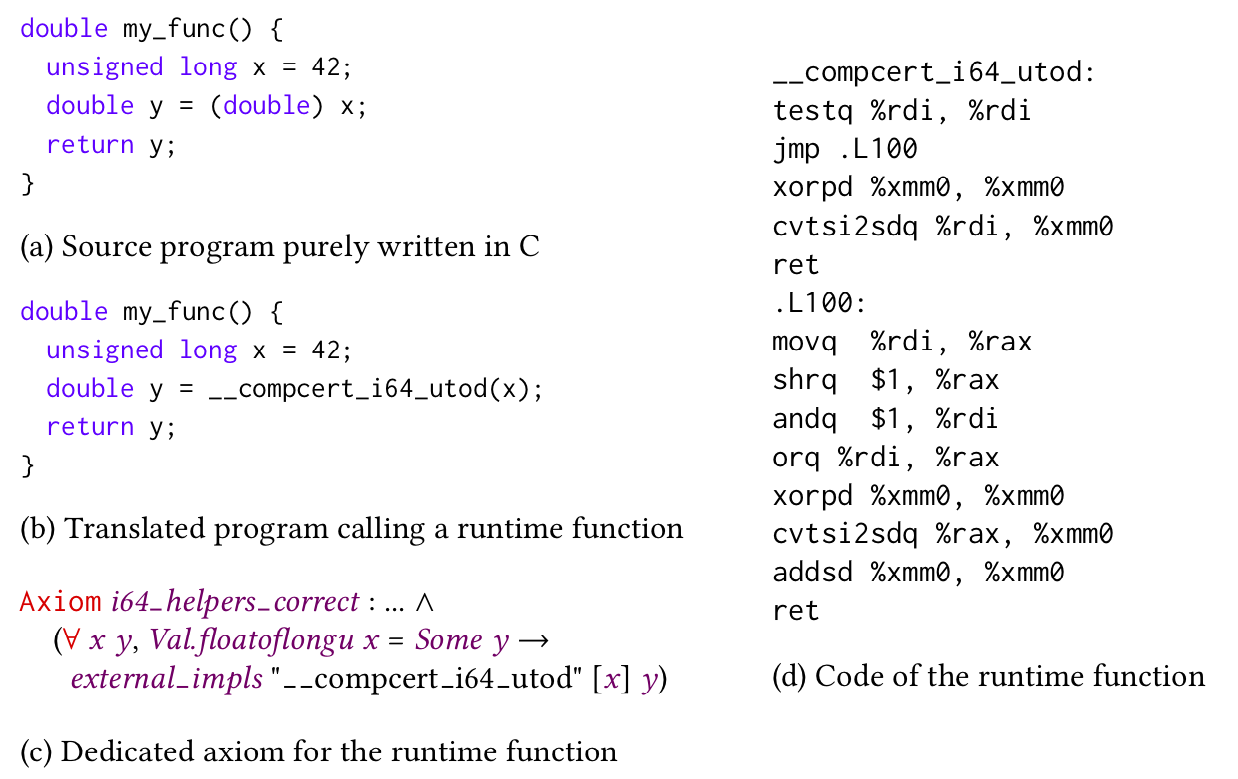
\includegraphics[width=1\linewidth]{images/utod.png}
%% \end{minipage}
%% }}
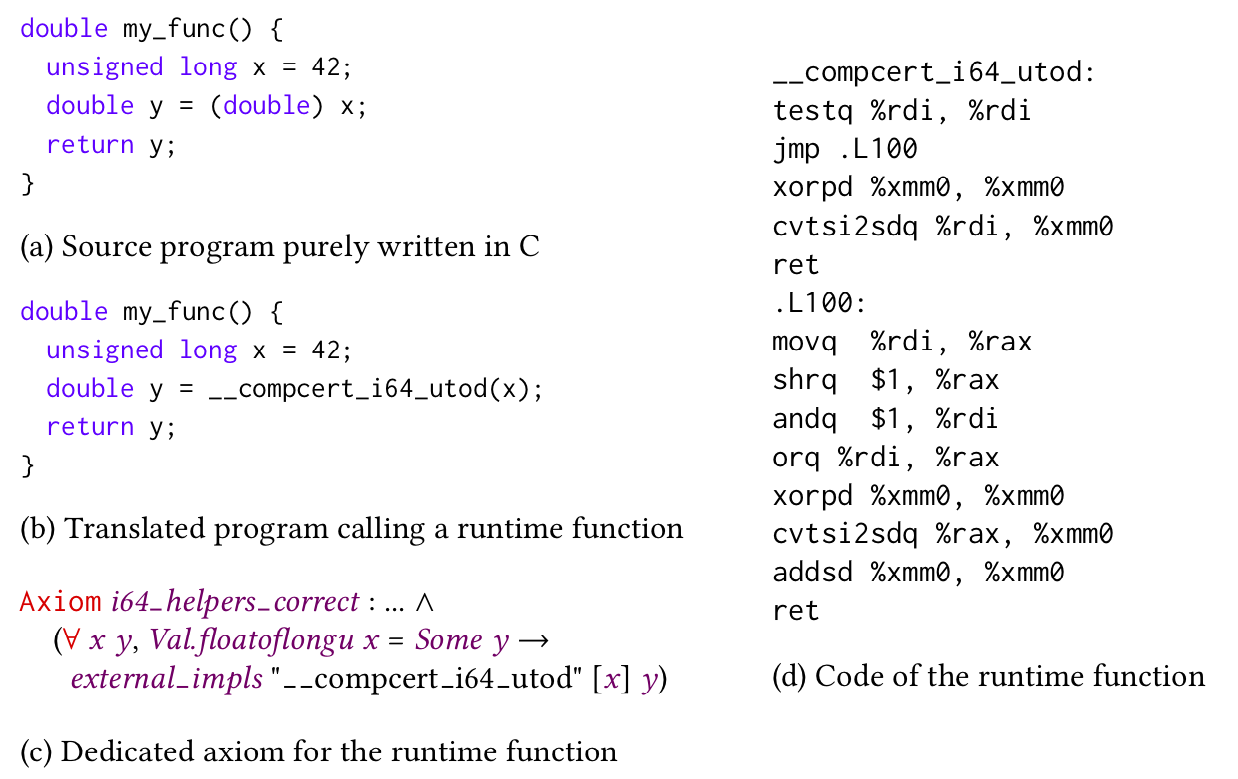
\includegraphics[width=1\linewidth]{images/utod.png}
\end{figure}

\[
\begin{minipage}{\textwidth}
\begin{coqdoccode}
\coqdocnoindent
\coqdockw{Axiom} \coqdoccst{i64\_helpers\_correct} : ... \ensuremath{\land}\coqdoceol
\coqdocindent{0.5em}
(\coqdockw{\ensuremath{\forall}} \coqdocvar{x} \coqdocvar{z}, \coqdocmod{Val}.\coqdoccst{floatoflongu} \coqdocvar{x} = \coqdocconstr{Some} \coqdocvar{z} \ensuremath{\rightarrow}
\coqdoccst{external\_implements} "\_\_compcert\_i64\_utod" \coqdoccst{sig\_l\_f} [\coqdocvar{x}] \coqdocvar{z})
\end{coqdoccode}
\end{minipage}
\]

We demonstrate that such axioms can be essentially removed in \ccm{} by proving the axiom for \verb|__compcert_i64_utod|.
We first turn the axiom for \verb|__compcert_i64_utod| into a specification module
and then establish an open simulation with memory injections between the assembly module containing \verb|__compcert_i64_utod| and the specification module.
}






\section{Comparison with Hoare Logic}
\label{sec:program:hoare}

\section{Future Works}
\label{sec:program:future}
%% automation 이야기... layered approach

%% \section{Background}
%% \label{sec:program:background}

%% \section{Problems}
%% \label{sec:program:problems}

%% \section{Solution}
%% \label{sec:program:solution}

\todo{put trimmed table from CompCertM}
